\documentclass[11pt]{ctexart}
\usepackage[utf8]{inputenc}
\usepackage{fontspec}
\usepackage{amsmath}
\usepackage{amssymb}
\usepackage{hyperref}
\usepackage[margin=1.2in]{geometry}
\usepackage{booktabs}
\usepackage{enumitem}
\usepackage{parskip}
\usepackage{setspace}
\usepackage{graphicx}
\usepackage[table]{xcolor}
\usepackage{pagecolor}
\usepackage{listings}

% Style rules
\setstretch{1.15}
\setcounter{secnumdepth}{0}
\date{}

% Dark mode styling
\definecolor{darkbg}{HTML}{1E1E1E}
\definecolor{lighttext}{HTML}{D4D4D4}
\pagecolor{darkbg}
\color{lighttext}

\hypersetup{
    colorlinks=true,
    linkcolor=cyan,
    citecolor=cyan,
    filecolor=cyan,
    urlcolor=cyan
}

% Code block styling
\lstset{
    backgroundcolor=\color{darkbg},
    basicstyle=\color{lighttext}\ttfamily\small,
    breaklines=true,
    frame=single,
    rulecolor=\color{lighttext},
    commentstyle=\color{gray},
    keywordstyle=\color{cyan},
    stringstyle=\color{orange}
}

\title{停止使用 AdamW，现在大家都在用 Muon}
\author{Vuk Rosić，由 Chaoqi Liang 审阅 \\ \small \raisebox{-0.2\height}{
\includegraphics[width=0.02\textwidth]{/Users/vukrosic/AI Science Projects/muon-course/.agent/skills/md-to-pdf/github.jpg}} \texttt{vukrosic/muon-optimizer-guide}}

\begin{document}
\maketitle

所有人（OpenAI, Meta, DeepSeek, Moonshot AI,...）都已经用 Muon 优化器替代了 AdamW 来训练他们的 LLMs 和神经网络。

DeepSeek 研究员表示，Muon 优化器是 2025 年最大的两项发明之一。

如果你训练任何神经网络 - 你必须尝试它！

它应该让你的训练速度提升 30\% 到 2 倍！

\subsection{Muon 击败 AdamW 的证据}

\begin{center}
    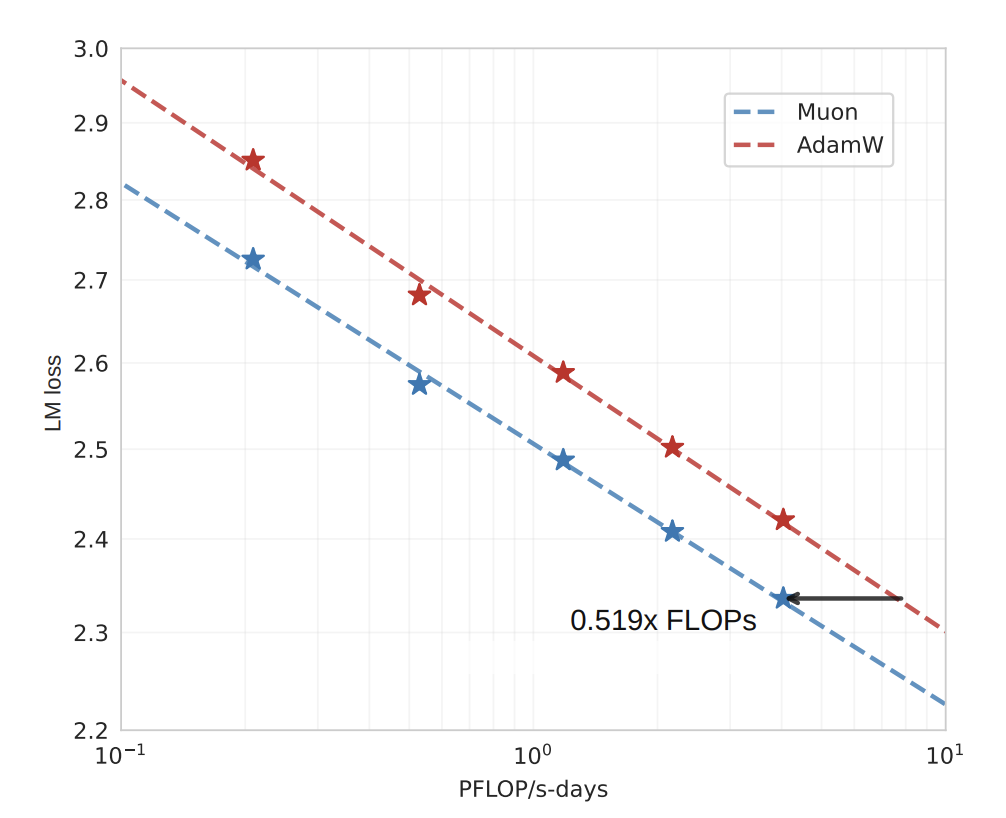
\includegraphics[width=0.8\textwidth]{images/muon_vs_adamw_kimi.png}
    
    图 1: \textit{Muon 在大规模 LLMs 上非常有效。} \href{https://arxiv.org/abs/2502.16982}{[MUON IS SCALABLE FOR LLM TRAINING on arxiv]}
\end{center}

不同的优化器以最少的 token 数最快地达到相同的损失：

\begin{center}
    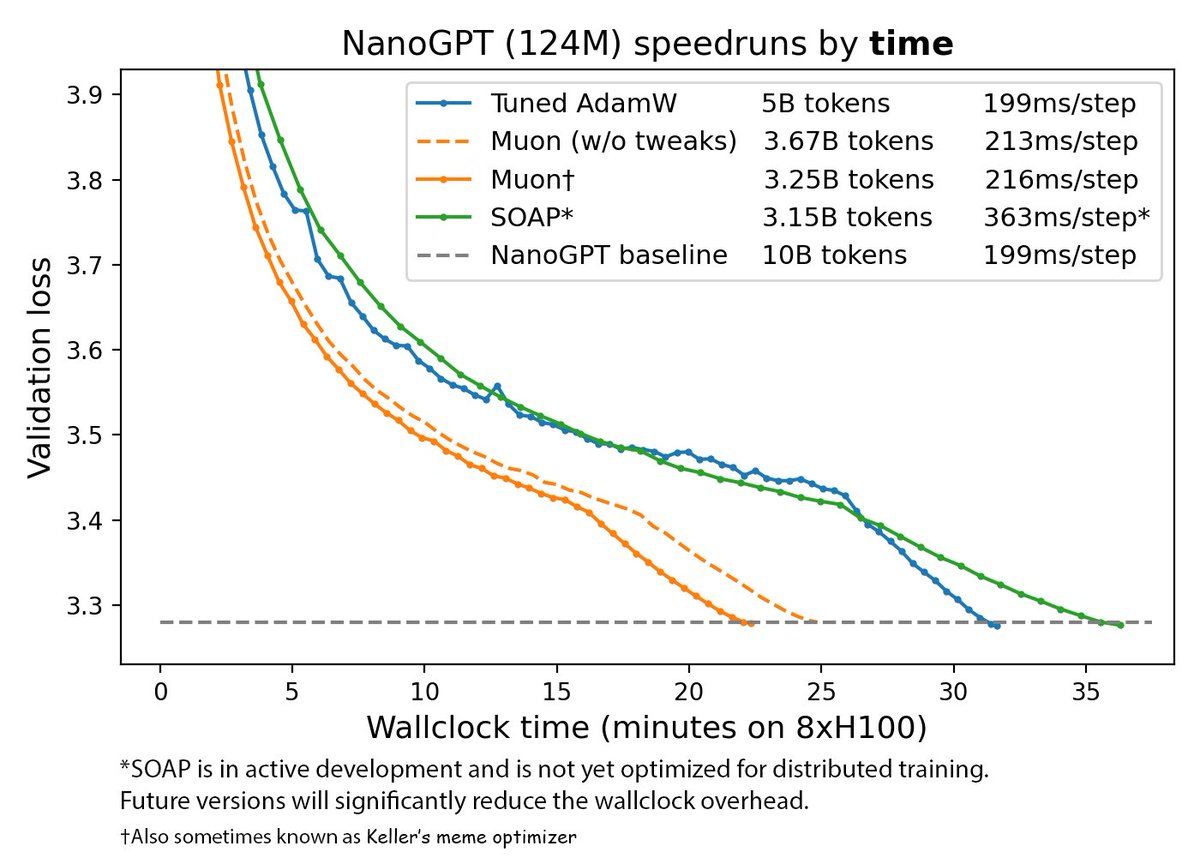
\includegraphics[width=0.8\textwidth]{images/nanogpt_curves.jpg}
    
    图 2: \textit{更快的 LLM 训练。} \href{https://kellerjordan.github.io/posts/muon/}{[Jordan et al. 2024]}
\end{center}

\begin{quote}
    关于代码与实现，请向下滚动查看。
\end{quote}

\section{核心思想}

如果你是一个初学者，看不懂这些，请将它复制到 Gemini, ChatGPT, Claude, Kimi 等，并让它教你。

让我们从参数更新的基本公式开始：

\[
\theta_{t+1} = \theta_t - \eta \cdot \nabla_{\theta} \mathcal{L}
\]

\begin{itemize}
    \item $\theta_t$: 在第 $t$ 步的模型参数（所有权重）。
    \item $\theta_{t+1}$: 一次训练步骤后更新的参数。
    \item $\eta$: 学习率（更新步长）。
    \item $\mathcal{L}$: 损失函数。
    \item $\nabla_{\theta} \mathcal{L}$: 损失对参数 $\theta$ 的梯度。
    \item $t$: 优化步数索引。
\end{itemize}

如果我们看一下梯度 $\nabla_{\theta} \mathcal{L}$，这个矩阵减去了权重 - 这就是神经网络学习的方式。然而，这个矩阵可能是病态（ill-conditioned）的 - 一些方向可能有较强的“拉力（pull）”，而其他方向可能有较弱的“拉力”。

\begin{center}
    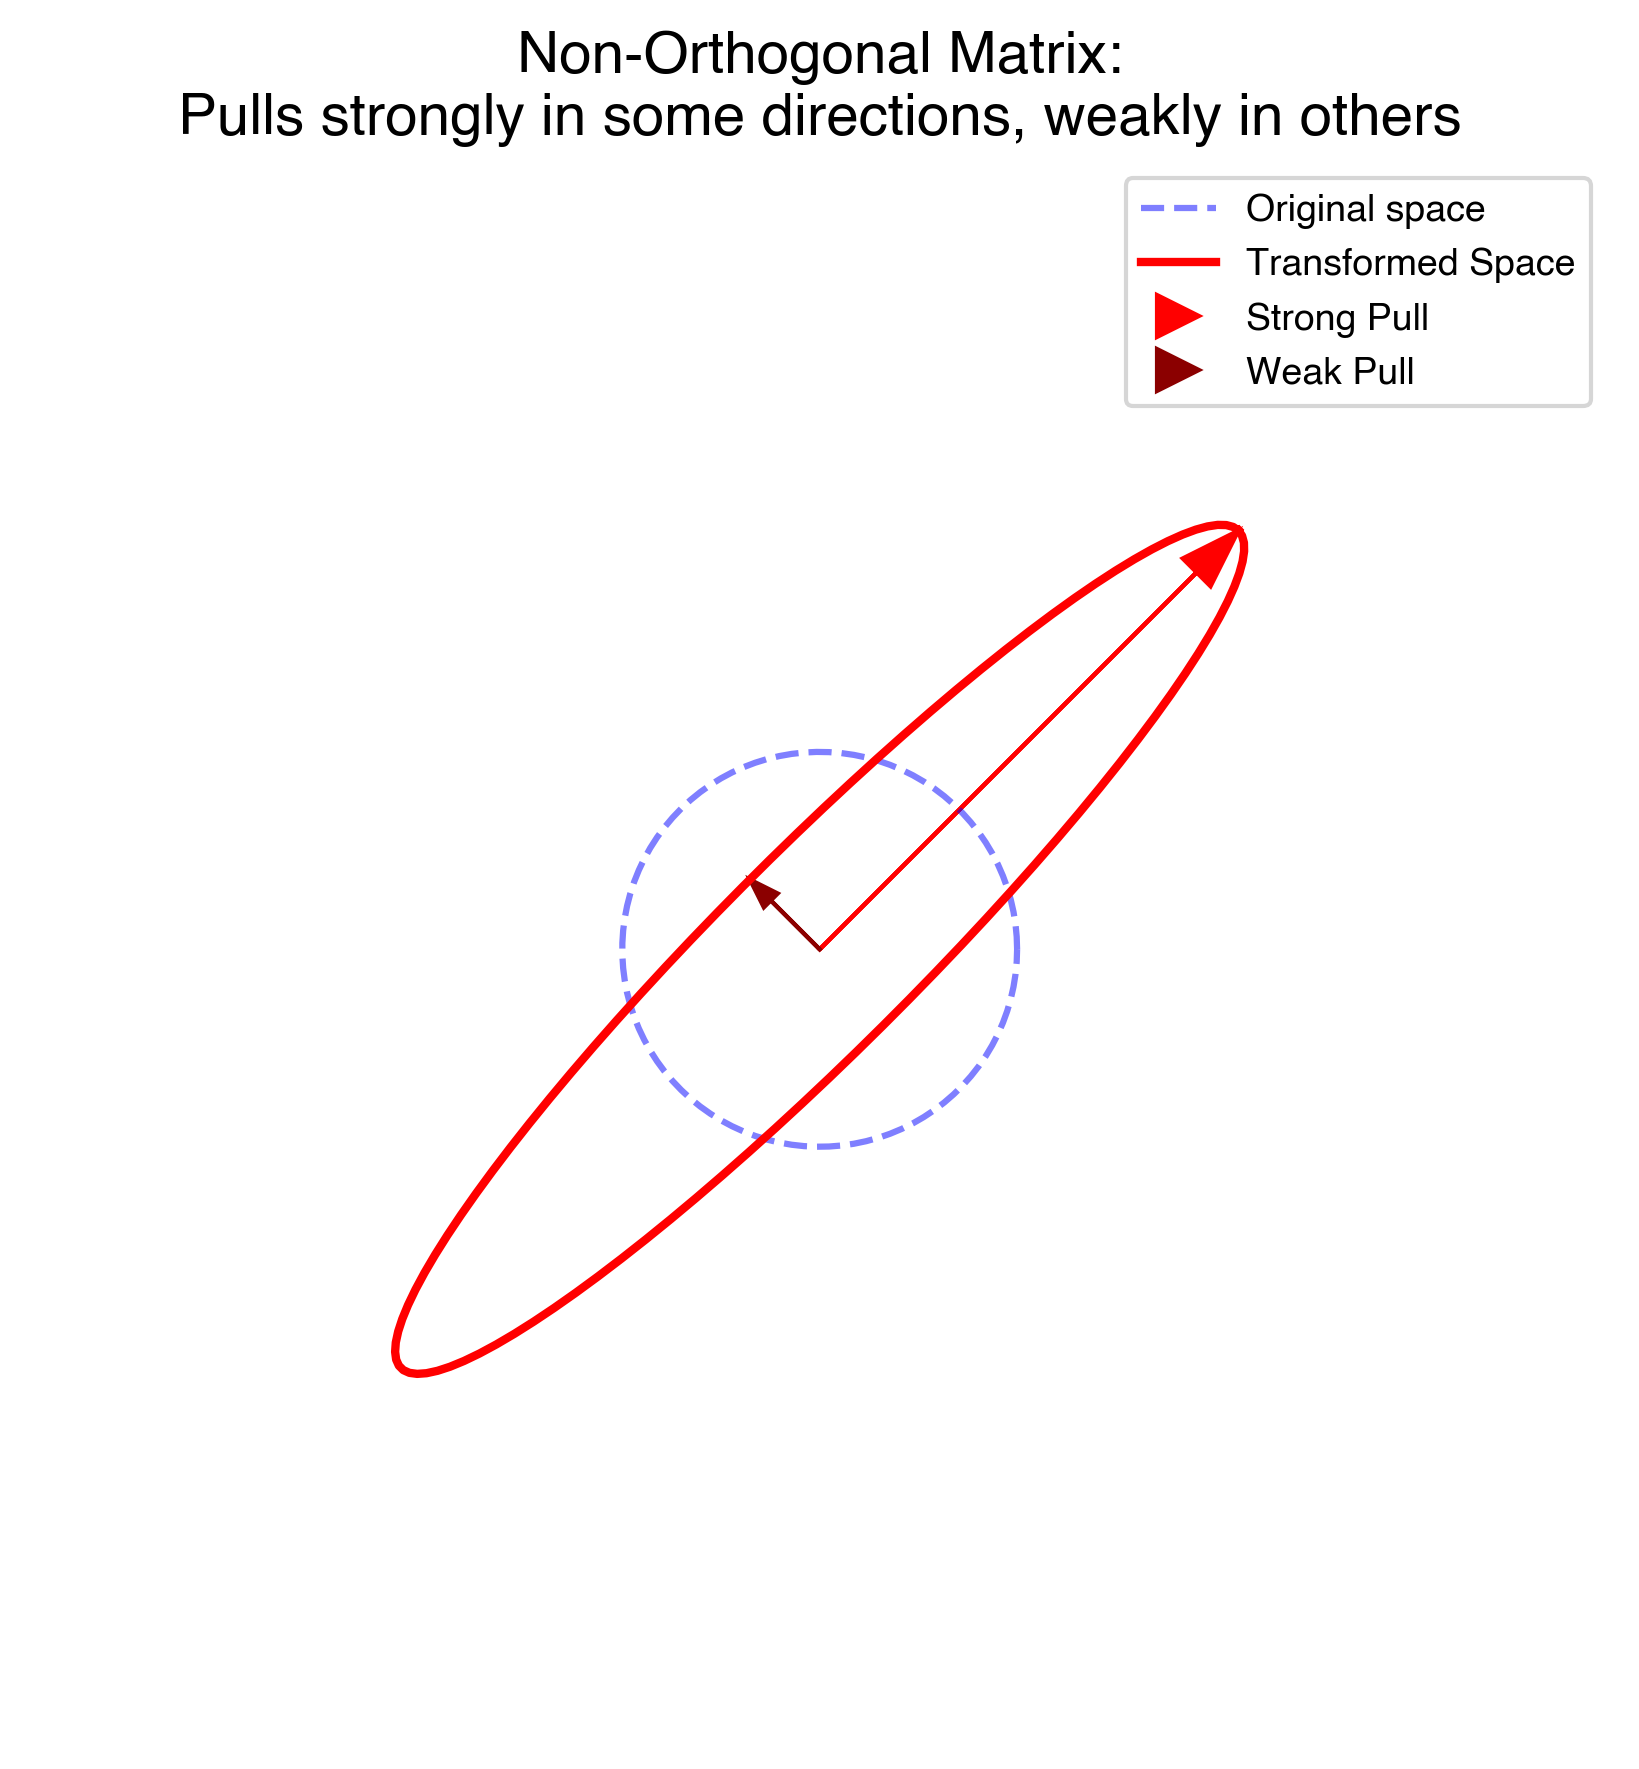
\includegraphics[width=0.8\textwidth]{images/01_non_orthogonal_effect.png}
    
    非正交效应 (Non-Orthogonal Effects)
\end{center}

“方向”或“拉力”跨越多个权重的协调变化。它控制了层中的 输入$\to$输出 路径。

例如：
假设我们正在训练一个神经网络 - 当它看到许多绿色时，应该预测“草地（grass）”，当它看到许多圆形时，应该预测“轮子（wheels）”。

由于不同类型的图像编码，绿色图像的梯度可能有非常小的奇异值（0.01），而圆形图像的梯度可能有较大的奇异值（100）。

这意味着神经网络学习 [绿色 $\to$ 草地] 路径（预测）的速度会比 [圆形 $\to$ 轮子] 路径慢得多。

并不是说关于绿色的数据更少或者圆形更重要，而仅仅是因为数据被表示为数字的方式造成的。

Muon 优化器解决了这个问题：

\begin{center}
    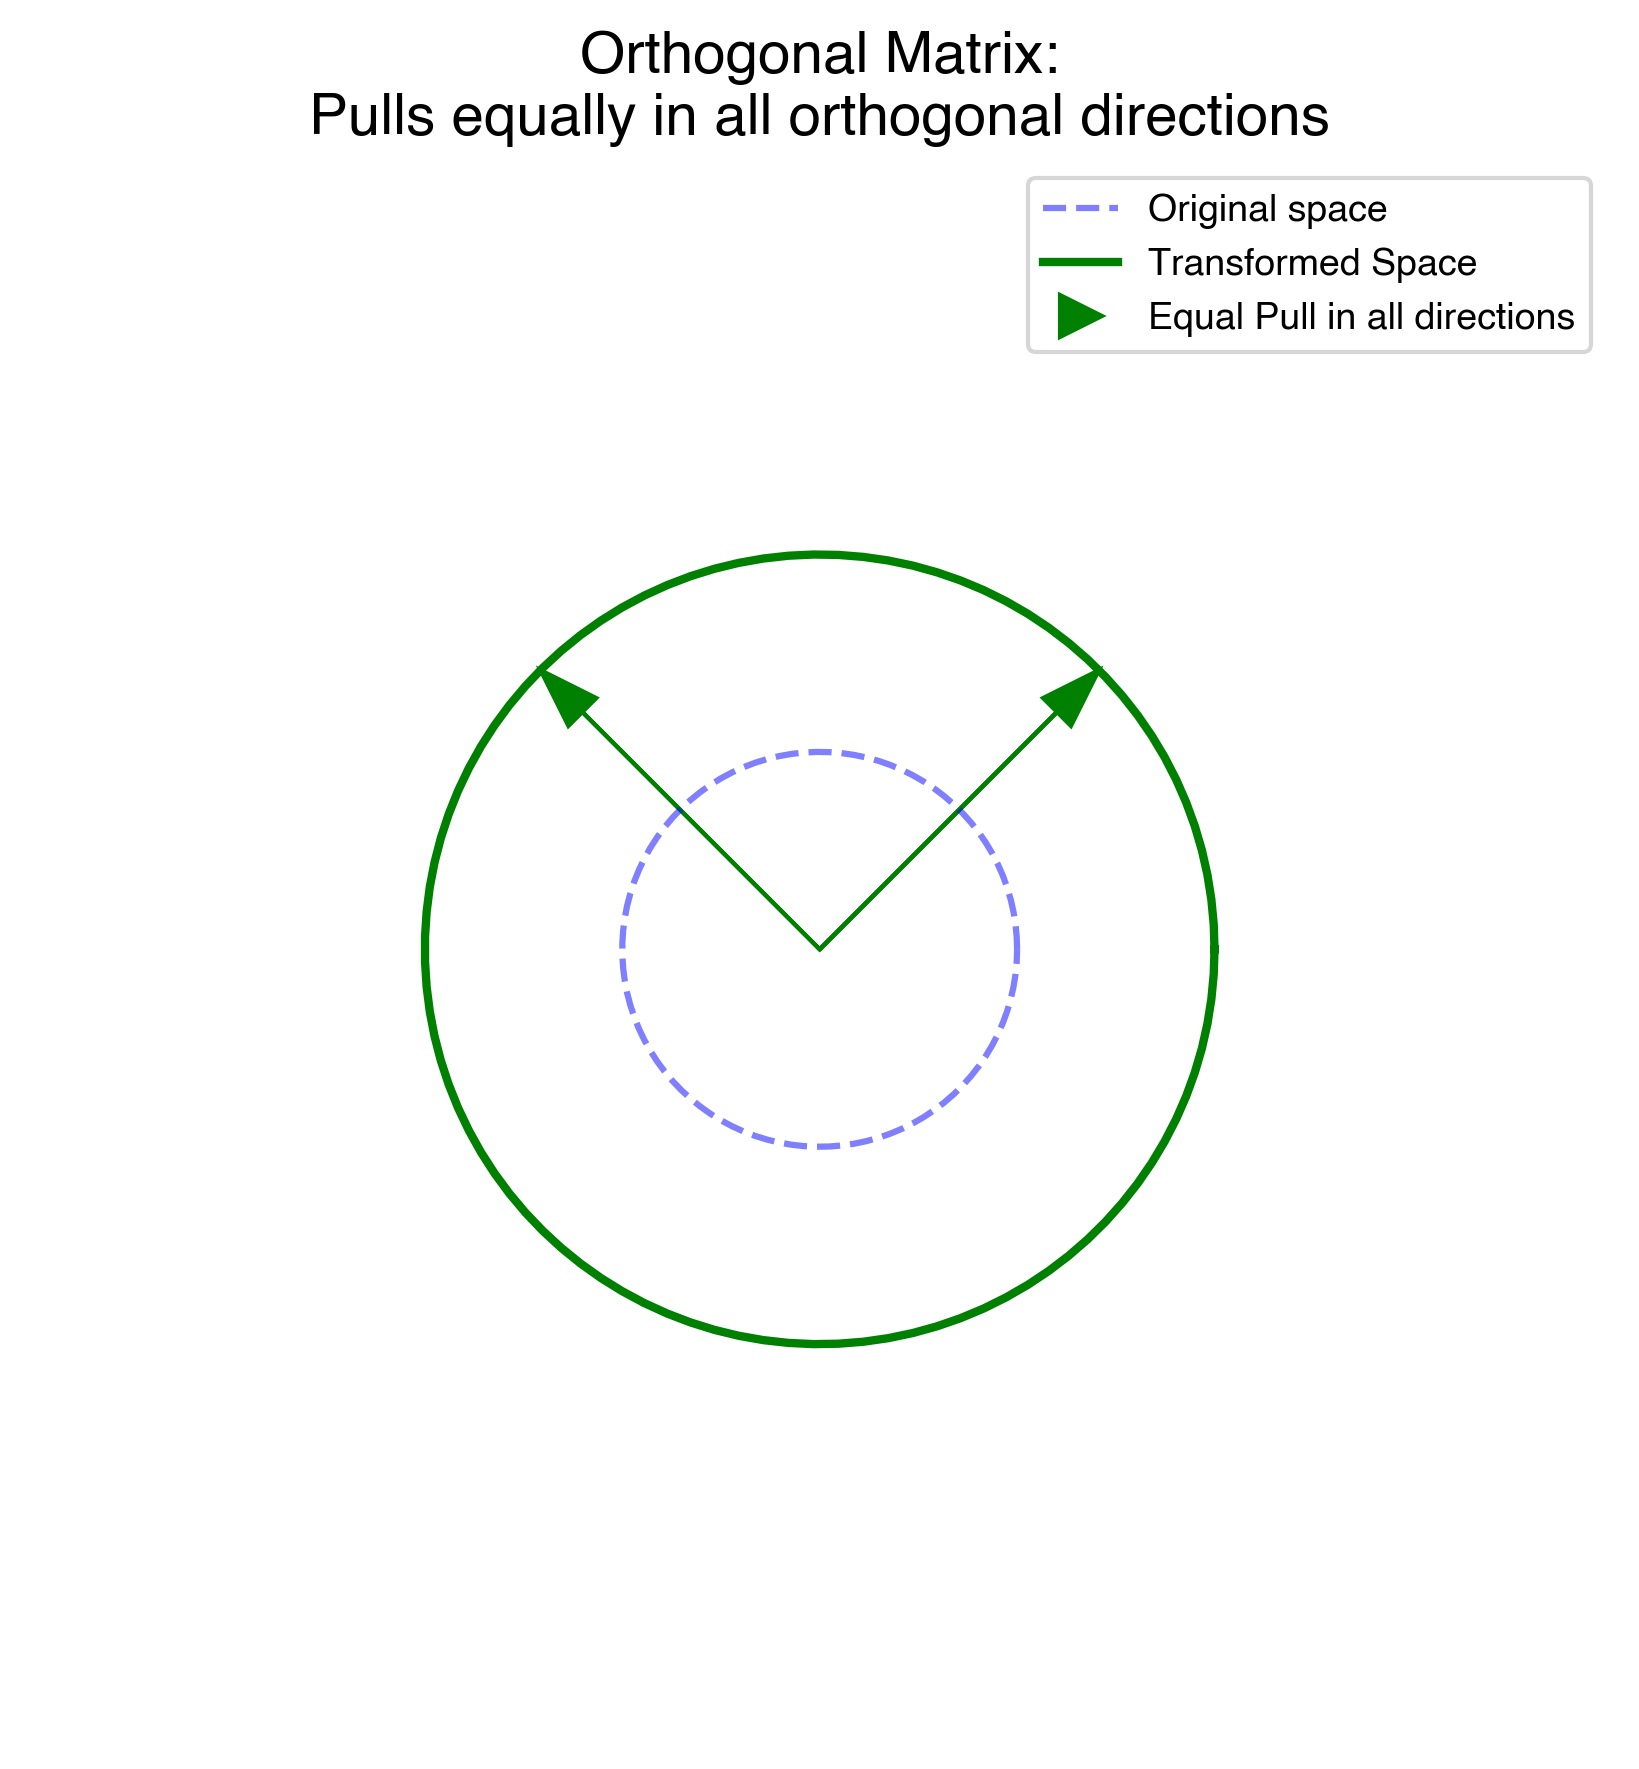
\includegraphics[width=0.8\textwidth]{images/01_orthogonal_effect.png}
    
    正交效应 (Orthogonal Effects)
\end{center}

\begin{center}
    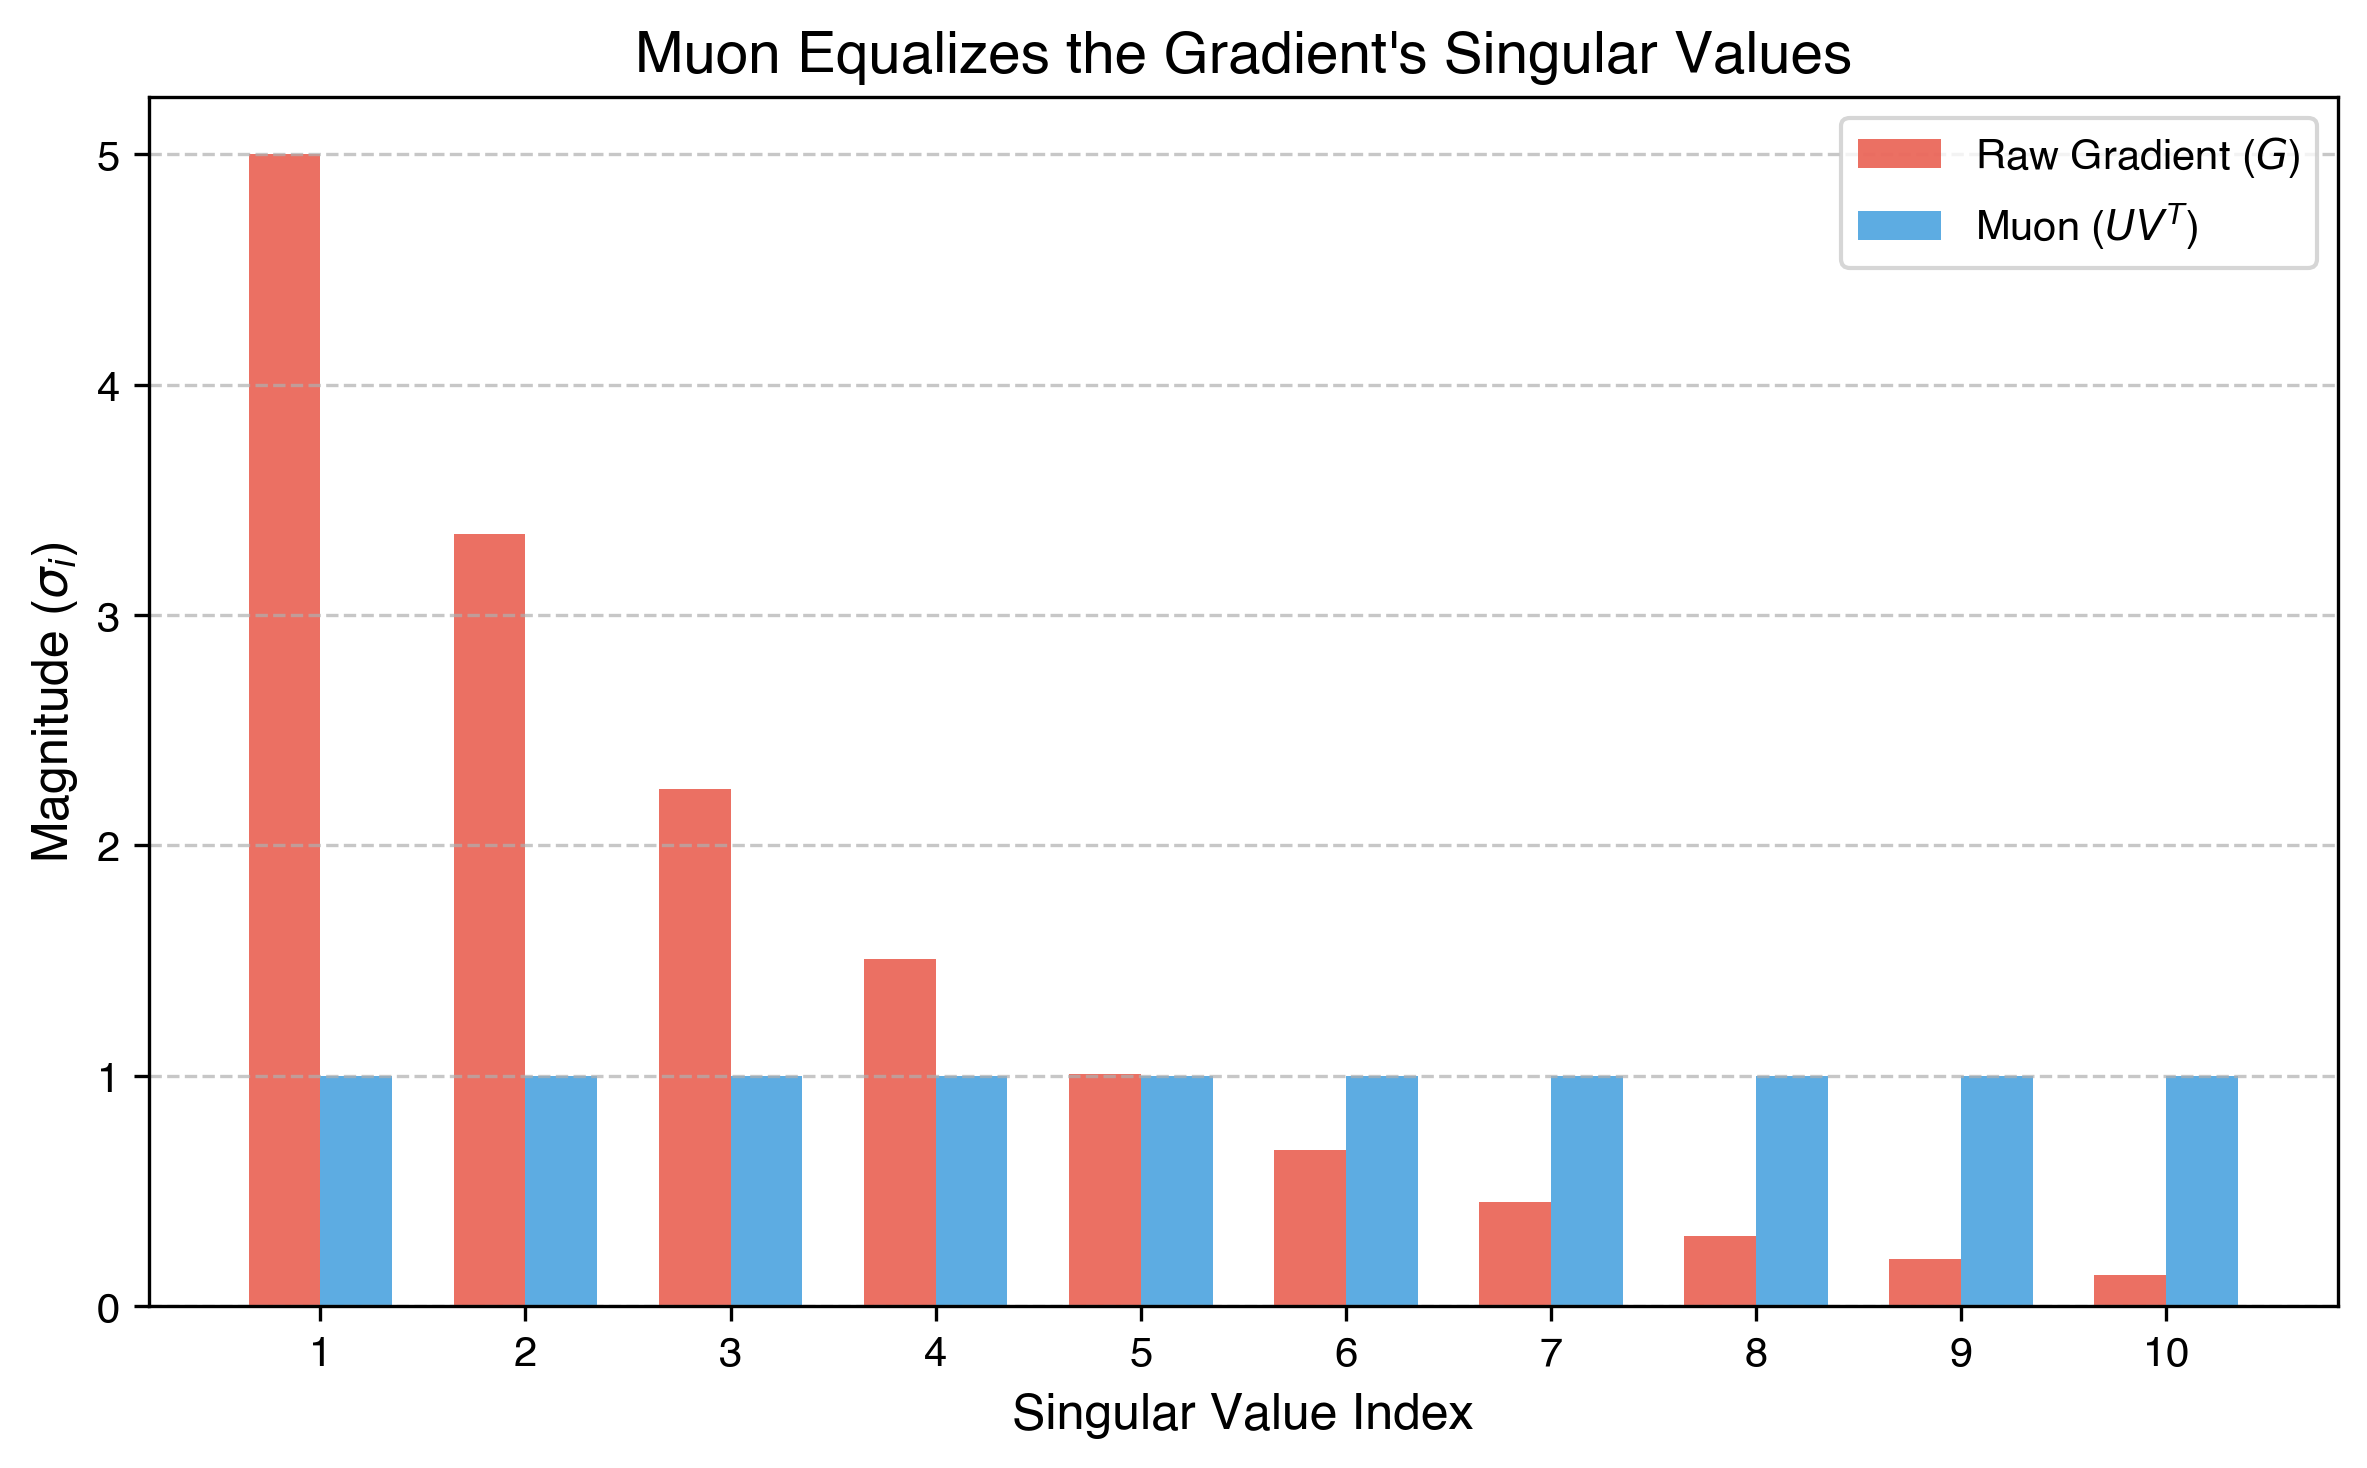
\includegraphics[width=0.8\textwidth]{images/03a_svd_for_muon_intro.png}
    
    Muon 的 SVD 直觉：原始梯度有不均匀的奇异值，而 Muon 使用带有等化奇异值的 UV\textsuperscript{T}。
\end{center}

Muon 优化器将使所有的奇异值等于 1（实际上接近 1，为了更快的计算速度），所以它在更新 / 学习 [绿色 $\to$ 草地] 路径时的速度将与 [圆形 $\to$ 轮子] 路径相同。

\textbf{重要}：仅将 Muon 用于 2D 权重矩阵。不要（Do NOT）将它用于 embeddings, biases, LayerNorms 或最终的输出头（output head）- 请使用 AdamW。

\subsubsection{关键区别}

Muon 优化器使得\textbf{权重更新矩阵（weight update matrices）}正交化，而非权重矩阵本身。

\section{代码与实现 (Code \& Implementation)}

通过 \href{https://github.com/KellerJordan/Muon/blob/master/muon.py}{搜索“muon keller jordan code”}可以找到原始的 Muon 代码。

下面我的实现包含了另一项改进 - \href{https://arxiv.org/abs/2505.16932}{polar express}。你也可以使用上面链接的原始代码，或者我的实现。

如果你将代码复制粘贴到你的 AI 代理中，它应该会自动实现它。

\begin{lstlisting}[language=Python]
import torch

# Polar Express coefficients - each step uses different, pre-optimized (a, b, c).
coeffs_list = [
    (8.156554524902461,  -22.48329292557795,   15.878769915207462),
    (4.042929935166739,  -2.808917465908714,    0.5000178451051316),
    (3.8916678022926607, -2.772484153217685,    0.5060648178503393),
    (3.285753657755655,  -2.3681294933425376,   0.46449024233003106),
    (2.3465413258596377, -1.7097828382687081,   0.42323551169305323),
]

@torch.compile()
def zeropower_polar_express(G: torch.Tensor, steps: int = 5) -> torch.Tensor:
    X = G.bfloat16()
    transposed = X.size(-2) > X.size(-1)
    if transposed:
        X = X.mT
    X = X / (X.norm(dim=(-2, -1), keepdim=True) * 1.01 + 1e-7)
    for a, b, c in coeffs_list[:steps]:
        A = X @ X.mT
        X = a * X + (b * A + c * A @ A) @ X
    return X.mT if transposed else X

class Muon(torch.optim.Optimizer):
    def __init__(self, params, lr: float = 0.02, momentum: float = 0.95,
                 weight_decay: float = 0.0):
        super().__init__(params, dict(lr=lr, momentum=momentum,
                                     weight_decay=weight_decay))

    @torch.no_grad()
    def step(self):
        for group in self.param_groups:
            for p in group["params"]:
                if p.grad is None:
                    continue
                state = self.state[p]
                if "buf" not in state:
                    state["buf"] = torch.zeros_like(p.grad)
                buf = state["buf"]
                buf.lerp_(p.grad, 1 - group["momentum"])
                g = p.grad.lerp_(buf, group["momentum"])
                g = zeropower_polar_express(g.view(g.size(0), -1))
                g = g.to(p.dtype)
                if group["weight_decay"] > 0:
                    p.mul_(1 - group["lr"] * group["weight_decay"])
                scale = max(1, p.size(-2) / p.size(-1)) ** 0.5
                p.add_(g.view_as(p), alpha=-group["lr"] * scale)
\end{lstlisting}

\begin{description}
    \item[注:] 为了快速使用，直接复制粘贴上面的代码即可。如果需要更多控制，请使用 \texttt{optimizers/muon.py}。
\end{description}

\subsection{使用示例 (Usage Example)}

\begin{lstlisting}[language=Python]
import torch
import torch.nn as nn

model = MyTransformer().cuda()

muon_params  = [p for p in model.parameters() if p.ndim == 2 and p.requires_grad]
adamw_params = [p for p in model.parameters() if not (p.ndim == 2 and p.requires_grad)]

optimizer_muon  = Muon(muon_params,  lr=0.02, momentum=0.95)
optimizer_adamw = torch.optim.AdamW(adamw_params, lr=3e-4, weight_decay=0.1)

for batch in dataloader:
    loss = model(batch)
    loss.backward()
    optimizer_muon.step()
    optimizer_adamw.step()
    optimizer_muon.zero_grad()
    optimizer_adamw.zero_grad()
\end{lstlisting}

\begin{description}
    \item[提示:] 一个简单的 \texttt{p.ndim == 2} 过滤器能够正确地分离出 Linear 层的权重矩阵。
\end{description}

\subsection{关键实现提示 (Key Implementation Tips)}

\subsubsection{使用大尺寸的学习率 (Use a BIG Learning Rate)}
不像通常使用 \texttt{3e-4} 的 AdamW，Muon 在使用大得多的学习率时表现最佳：
\begin{itemize}
    \item \textbf{默认 (Default):} \texttt{0.02}。
    \item \textbf{范围 (Range):} \texttt{0.01} 到 \texttt{0.05}。
\end{itemize}

\subsubsection{参数路由 (Parameter Routing)}
Muon 仅专为 2-D 权重矩阵设计。请将 AdamW 用于所有其他参数上。

\subsubsection{编译它！ (Compile It!)}
为了性能，请使用 \texttt{@torch.compile()}。

\subsubsection{根据矩阵形状缩放学习率 (Scaling the LR by Matrix Shape)}
此更新由 $\sqrt{\max(1, \text{rows} / \text{cols})}$ 缩放。

\end{document}
